\documentclass[11pt,a4paper]{article}
\usepackage[T1]{fontenc}
\usepackage{lmodern}
\usepackage{microtype}
\usepackage[margin=2.2cm]{geometry}
\usepackage{amsmath,amssymb}
\usepackage{graphicx}
\usepackage{booktabs}
\usepackage{tabularx}
\usepackage{array}
\usepackage[table]{xcolor}
\usepackage{enumitem}
\usepackage{placeins}
\usepackage[font=small,labelfont=bf]{caption}
\usepackage[most]{tcolorbox}
\usepackage[colorlinks=true,linkcolor=blue!50!black,urlcolor=blue!50!black]{hyperref}

\graphicspath{{figures/}}
\setlist{nosep,leftmargin=*}
\setlength{\parskip}{4pt}
\setlength{\parindent}{0pt}
\newcolumntype{L}{>{\raggedright\arraybackslash}X}
\newtcolorbox{keybox}[1]{colback=blue!3,colframe=blue!40!black,boxrule=0.5pt,arc=1pt,
  left=6pt,right=6pt,top=4pt,bottom=4pt,title={#1},fonttitle=\bfseries\small}
\newtcolorbox{failbox}[1]{colback=red!3,colframe=red!45!black,boxrule=0.5pt,arc=1pt,
  left=6pt,right=6pt,top=4pt,bottom=4pt,title={#1},fonttitle=\bfseries\small}
\newcommand{\code}[1]{\texttt{\footnotesize #1}}

\title{\textbf{The two plate models used in Hybrid-OED}\\[4pt]
\large Plane stress (S0/SH0) and Mindlin (A0): physics, variables, failure mechanisms and corrections}
\author{Technical note, companion to the October 2026 status report}
\date{}

\begin{document}
\maketitle

\begin{keybox}{In one paragraph}
A 10~mm plate guides elastic waves. Between 10 and 50~kHz only three wave types (\emph{modes}) exist: \textbf{S0}
(in-plane stretching), \textbf{SH0} (in-plane shearing) and \textbf{A0} (bending). A plate model replaces the 3-D
elasticity of the thickness by an assumed through-thickness motion, which turns the problem into a 2-D one and makes
it cheap. \textbf{Plane stress} assumes the in-plane motion is uniform through the thickness: it carries S0 and SH0 and
cannot carry A0. \textbf{Mindlin} assumes the plate bends with straight (but not necessarily perpendicular) normals: it
carries A0 and nothing else. Each is accurate only if (i) its assumed motion matches the real mode shape, (ii) its
wave speed is calibrated to the exact one (otherwise small speed errors accumulate into large waveform misfits), and
(iii) whatever the plate is attached to or excited by is represented in its own variables. The corrections used in
the project address exactly these three points.
\end{keybox}

\tableofcontents

%======================================================================
\section{Guided waves in a plate: what a ``mode'' is}
In a plate the wave field at a point is a superposition of \emph{modes}. A mode is a wave that travels along the
plate with a \emph{fixed shape through the thickness} and its own speed, which depends on frequency
(\emph{dispersion}). For a free plate of thickness $h$, bulk speeds $v_p, v_s$, the modes follow from the
Rayleigh--Lamb equations (Lamb waves) plus the shear-horizontal (SH) family. They split into:
\begin{itemize}
  \item \textbf{symmetric} modes (S0, S1, \ldots): in-plane motion symmetric about the mid-plane, the plate stretches and
        compresses; S0 at low frequency is a ``membrane'' wave at the plate velocity
        $c_p = \sqrt{E/(\rho(1-\nu^2))} = 2v_s\sqrt{1 - v_s^2/v_p^2}$;
  \item \textbf{antisymmetric} modes (A0, A1, \ldots): the plate bends; A0 is the \emph{flexural} wave, slow and strongly
        dispersive (its speed grows roughly like $\sqrt{f}$ at low frequency);
  \item \textbf{shear-horizontal} modes (SH0, SH1, \ldots): in-plane motion perpendicular to the propagation direction;
        SH0 is non-dispersive and travels exactly at $v_s$.
\end{itemize}
For the 10~mm PMMA plate (vp 2730, vs 1340~m/s), the first higher modes (A1, SH1) appear at $f = v_s/(2h) = 67$~kHz.
Below that, only \textbf{S0, SH0 and A0} propagate (Fig.~\ref{fig:disp}). This is what makes 2-D plate models possible:
each of them only needs to reproduce one or two of these three modes.

\begin{figure}[h]
\centering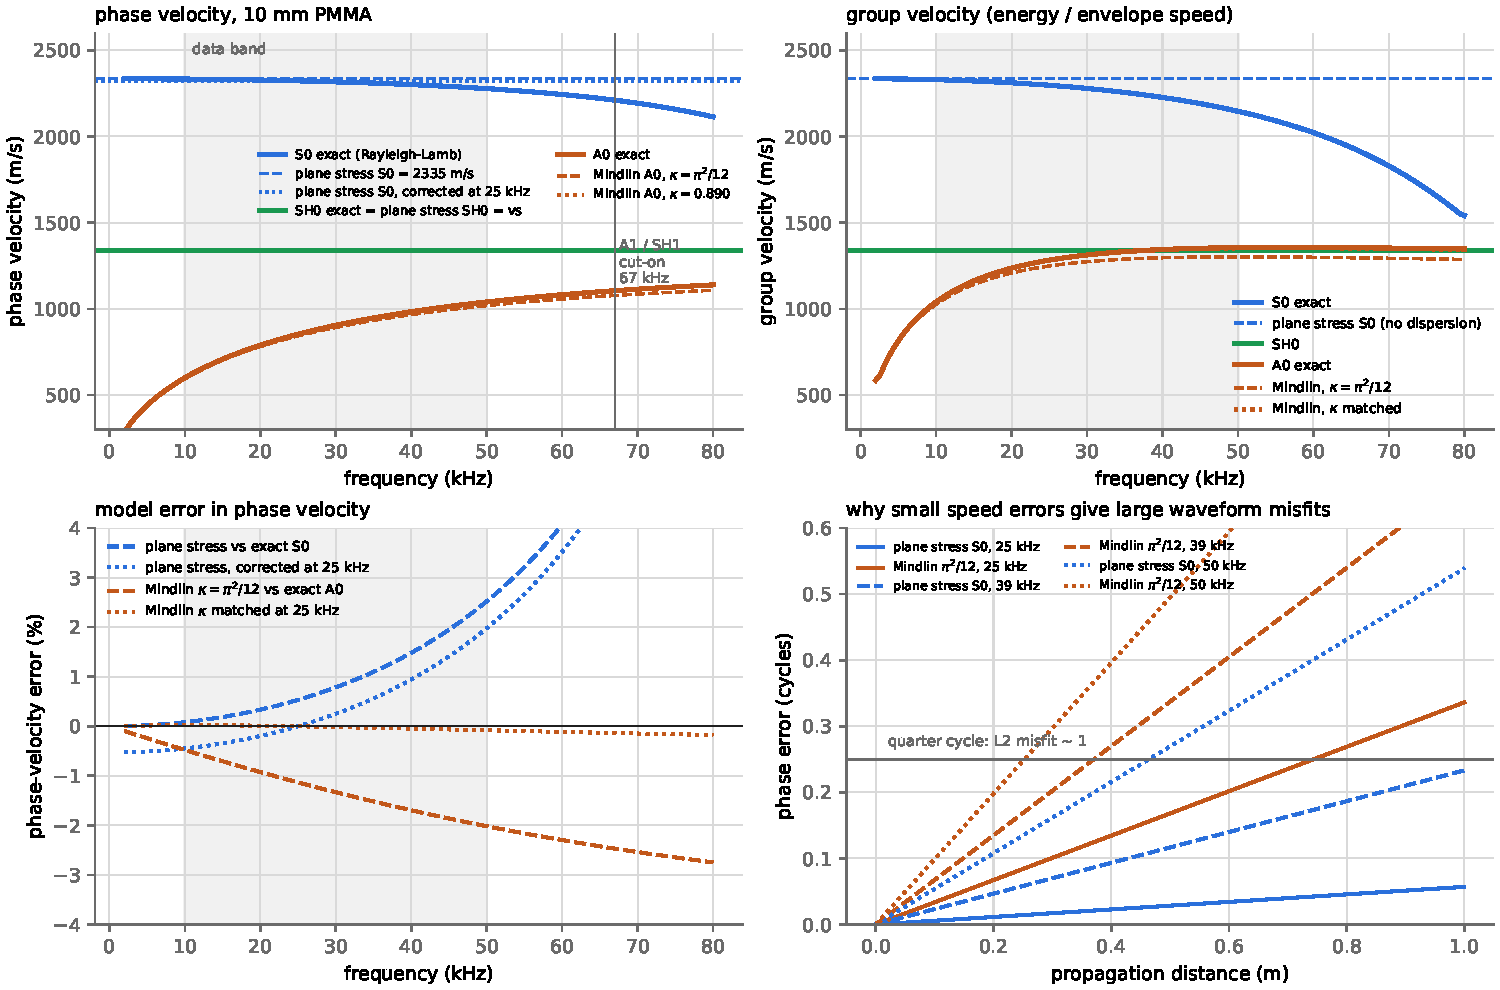
\includegraphics[width=\textwidth]{dispersion.pdf}
\caption{\label{fig:disp}10~mm PMMA. Top: phase and group velocities of the exact modes (solid) and of the plate
models (dashed: uncorrected, dotted: corrected). Bottom left: model phase-velocity errors. Bottom right: phase error,
in cycles, accumulated over a propagation distance; a quarter cycle already makes the L2 waveform misfit of order one.
The grey band is the data band (10--50~kHz).}
\end{figure}

\begin{figure}[h]
\centering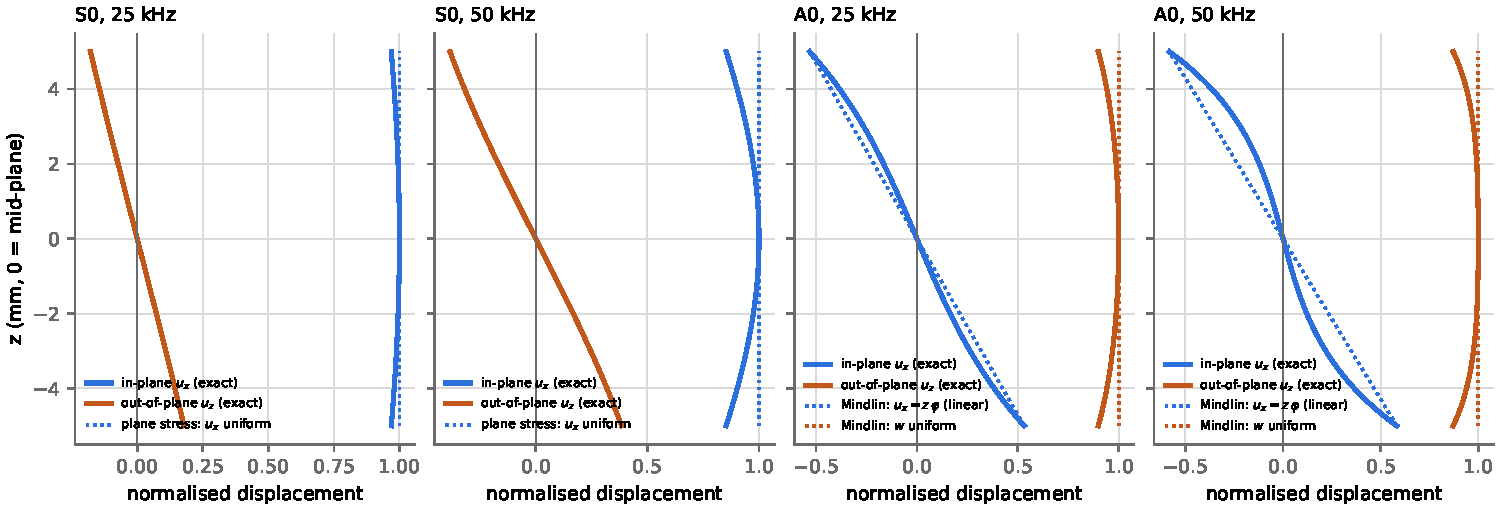
\includegraphics[width=\textwidth]{mode_shapes.pdf}
\caption{\label{fig:shapes}Exact through-thickness displacement of S0 and A0 (solid), and what the plate models assume
(dotted). S0: nearly uniform in-plane motion plus a small linear thickness ``breathing'' $u_z$ (Poisson effect);
plane stress assumes exactly this. A0: nearly uniform deflection $w$ and in-plane motion linear in $z$ (rotation of
the normal); Mindlin assumes exactly this. At 50~kHz the exact shapes start to curve: this is where the models start
to need corrections.}
\end{figure}

\subsection*{Which modes a source excites and a sensor sees}
\begin{table}[h]
\centering\small
\begin{tabularx}{\textwidth}{@{}>{\raggedright\arraybackslash}p{6.2cm}L@{}}
\toprule
Excitation / measurement & Modes \\
\midrule
In-plane force at mid-plane (Salvus in-plane benchmark) & S0 + SH0 only (symmetric load) \\
Normal force at mid-plane (Salvus flexural benchmark) & A0 only (antisymmetric load) \\
Normal force on one surface (transducer, LDV experiment) & mostly A0, plus a weaker S0 part (a one-sided load = half symmetric, half antisymmetric) \\
Object bonded on one surface (steel cube) & couples all: it adds mass and rotary inertia above the plate \\
Out-of-plane velocity on the surface (LDV $v_z$) & A0 (large) + S0 breathing (small) \\
In-plane velocity on the surface & S0 + SH0 + the A0 rotation part $\pm(h/2)\,\varphi$ \\
\bottomrule
\end{tabularx}
\end{table}
This table explains two observations of the project: the real LDV data are A0-dominated (transducer on the surface,
out-of-plane measurement), and plane stress could therefore not be used for them.

\FloatBarrier
%======================================================================
\section{Plane-stress model (S0 and SH0)}
\subsection{Assumptions and equations}
The plate is treated as a membrane: the stresses acting on planes parallel to the surfaces vanish,
$\sigma_{zz} = \sigma_{xz} = \sigma_{yz} = 0$, and the in-plane displacement is uniform through the thickness.
The thickness change follows from the Poisson effect. Eliminating $\sigma_{zz}$ gives the plane-stress moduli
\[
\lambda^{*} = \frac{2\lambda\mu}{\lambda + 2\mu}, \qquad M = \lambda^{*} + 2\mu = \frac{E}{1-\nu^2},
\]
and the velocity--stress equations solved in \code{src/elastic/plane\_stress.py}
(functions \code{plane\_stress\_cpml} and \code{plane\_stress\_free}):
\[
\rho\,\dot v_x = \partial_x\sigma_{xx} + \partial_y\sigma_{xy} + f_x, \quad
\rho\,\dot v_y = \partial_x\sigma_{xy} + \partial_y\sigma_{yy} + f_y,
\]
\[
\dot\sigma_{xx} = M\,\partial_x v_x + \lambda^{*}\partial_y v_y, \quad
\dot\sigma_{yy} = \lambda^{*}\partial_x v_x + M\,\partial_y v_y, \quad
\dot\sigma_{xy} = \mu(\partial_y v_x + \partial_x v_y).
\]
It supports exactly two waves: SH0 at $v_s$ (exact) and S0 at the constant plate velocity $c_p$ (2335~m/s here).

\subsection{Variables}
\begin{table}[h]
\centering\small
\begin{tabularx}{\textwidth}{@{}llL@{}}
\toprule
Variable & Grid position & Physical meaning \\
\midrule
$v_x, v_y$ & $(i-\tfrac12, j)$, $(i, j-\tfrac12)$ & in-plane particle velocity, same at every depth (m/s); what is compared with surface in-plane data \\
$\sigma_{xx}, \sigma_{yy}$ & nodes $(i,j)$ & in-plane normal stresses (Pa, per unit thickness) \\
$\sigma_{xy}$ & $(i-\tfrac12, j-\tfrac12)$ & in-plane shear stress \\
$v_p, v_s, \rho$ & nodes & material maps; $v_s$ is the inversion parameter \\
$f_x, f_y$ & bilinear at the source & in-plane point force (per unit thickness: 2-D and 3-D amplitudes differ by a constant) \\
\bottomrule
\end{tabularx}
\end{table}
Edges: CPML (open plate) or traction-free edges by stress imaging (normal stress zero on the edge nodes, shear stress
antisymmetric across the edge). Grid: 1~mm, 1.4~s per 1~ms simulation on the GPU.

\subsection{Failure mechanisms}
\begin{failbox}{When plane stress fails, and why}
\begin{enumerate}
  \item \textbf{S0 is dispersive in reality, not in the model.} The exact S0 slows down with frequency (0.5\,\% at
        25~kHz, 2.5\,\% at 50~kHz for 10~mm PMMA, Fig.~\ref{fig:disp}). A constant model speed means a phase error
        that grows linearly with propagation distance; after many edge reverberations it reaches a sizeable fraction
        of a cycle and the L2 misfit grows with time (0.23 at 300~$\mu$s $\to$ 0.38 at 1~ms in the benchmark).
  \item \textbf{No A0.} Any one-sided excitation (surface transducer), one-sided defect (bonded object, surface
        corrosion) or out-of-plane measurement involves A0, which the model cannot produce. This is why the LDV data
        could not be used with plane stress.
  \item \textbf{Surface in-plane data contain A0.} A sensor on the surface sees the A0 rotation term
        $\pm(h/2)\varphi$ on top of the membrane motion.
  \item \textbf{Through-thickness variations are averaged.} An inclusion that varies through the thickness must be
        replaced by thickness-averaged membrane moduli; if it is not symmetric about the mid-plane it also couples
        stretching and bending, which the model ignores.
  \item \textbf{2-D point source vs 3-D point force.} Amplitudes differ by a constant (force per unit thickness), and
        the near field within a few thicknesses of the source is not 3-D.
  \item \textbf{Above 67~kHz} higher modes (A1, SH1) exist and no two-mode plate theory applies.
\end{enumerate}
\end{failbox}

\subsection{Corrections used}
\begin{itemize}
  \item \textbf{S0 dispersion correction} (\code{s0\_corrected\_vp}): keep $v_s$ (SH0 is exact) and replace $v_p$ by the
        value for which $c_p$ equals the exact Rayleigh--Lamb S0 phase velocity at the centre frequency (25~kHz:
        2322.6 instead of 2334.9~m/s). Effect on the benchmark misfit: 0.38 $\to$ 0.27 at 1~ms, 0.23 $\to$ 0.18 early.
        It is exact at one frequency only (Fig.~\ref{fig:disp}, bottom left); the residual frequency-dependent part
        is what remains.
  \item \textbf{Amplitude scale}: one factor per source, solved in closed form inside the misfit (variable projection).
  \item \textbf{Shorter windows} (300--500~$\mu$s) where the accumulated phase error is still small.
\end{itemize}

\FloatBarrier
%======================================================================
\section{Mindlin plate model (A0)}
\subsection{Assumptions and equations}
The plate bends; a line normal to the mid-plane stays straight but may tilt relative to the deflected mid-plane
(\emph{shear deformation}), and its rotation has inertia (\emph{rotary inertia}). With $w$ the deflection and
$\varphi_x, \varphi_y$ the rotations of the normal, the displacement at height $z$ above the mid-plane is
\[
u_x = z\,\varphi_x, \quad u_y = z\,\varphi_y, \quad u_z = w ,
\]
which is the A0 shape of Fig.~\ref{fig:shapes}. The resultants (per unit width) are bending/twisting moments
$M_{xx}, M_{yy}, M_{xy}$ and transverse shear forces $Q_x, Q_y$. In velocity form ($v_z = \dot w$,
$\Omega = \dot\varphi$), as solved by \code{mindlin\_plate} (\code{src/elastic/mindlin.py}):
\[
\rho h\,\dot v_z = \partial_x Q_x + \partial_y Q_y + q, \qquad
\rho I\,\dot\Omega_x = \partial_x M_{xx} + \partial_y M_{xy} - Q_x, \qquad I = h^3/12,
\]
\[
\dot M_{xx} = D(\partial_x\Omega_x + \nu\,\partial_y\Omega_y), \quad
\dot M_{xy} = D\,\tfrac{1-\nu}{2}(\partial_y\Omega_x + \partial_x\Omega_y), \quad
\dot Q_x = \kappa G h\,(\partial_x v_z + \Omega_x),
\]
(and the $y$ equations by symmetry), with bending stiffness $D = E h^3/(12(1-\nu^2))$, shear stiffness $\kappa G h$ and
\textbf{shear correction factor} $\kappa$. The plane-wave dispersion relation is a quadratic in $k^2$:
\[
(\kappa G h\,k^2 - \rho h\,\omega^2)(D k^2 + \kappa G h - \rho I\,\omega^2) - (\kappa G h)^2 k^2 = 0 .
\]
One root is A0. The other branch is a thickness-shear wave with cut-on frequency
$f_c = \sqrt{12\kappa}\,v_s/(2\pi h)$; Mindlin's original choice $\kappa = \pi^2/12$ places it exactly at the exact
A1 cut-on (67~kHz).

\subsection{Variables}
\begin{table}[h]
\centering\small
\begin{tabularx}{\textwidth}{@{}llL@{}}
\toprule
Variable & Grid position & Physical meaning \\
\midrule
$v_z$ & nodes $(i,j)$ & deflection velocity, the same at every depth; \textbf{what the LDV measures} (out-of-plane) \\
$\Omega_x, \Omega_y$ & $(i-\tfrac12, j)$, $(i, j-\tfrac12)$ & rotation rates of the normal (rad/s); top-surface in-plane velocity $= (h/2)\,\Omega$ \\
$M_{xx}, M_{yy}$ & nodes & bending moments per unit width (N) \\
$M_{xy}$ & $(i-\tfrac12, j-\tfrac12)$ & twisting moment \\
$Q_x, Q_y$ & with $\Omega_x$, $\Omega_y$ & transverse shear forces per unit width (N/m) \\
$\rho h,\ \rho I,\ D,\ \kappa G h$ & nodes / faces & mass, rotary inertia, bending and shear stiffness per unit area; can be scaled locally (\code{mass\_scale}, \code{inertia\_scale}, \code{stiffness\_scale}) \\
$q$ & bilinear at the source & normal point force (transducer) \\
\bottomrule
\end{tabularx}
\end{table}
Edges: traction-free ($M_{nn} = M_{ns} = Q_n = 0$, same imaging approach as plane stress) or an absorbing sponge.
Grid: 0.5~mm (A0 wavelengths are about half those of S0), 5--10~s per simulation on the GPU.

\subsection{Failure mechanisms}
\begin{failbox}{When Mindlin fails, and why}
\begin{enumerate}
  \item \textbf{A0 speed error from $\kappa$.} With $\kappa = \pi^2/12$ the model A0 is 1.1\,\% too slow at 25~kHz
        and 2\,\% at 50~kHz (Fig.~\ref{fig:disp}). The accumulated phase error reaches a quarter cycle within
        0.3--0.6~m, and the benchmark misfit was 0.87--0.99, i.e.\ no fit at all, although arrivals and shapes looked
        right.
  \item \textbf{No S0.} A load on one surface also creates the symmetric breathing part (S0) visible in $v_z$; Mindlin
        lacks it (total misfit 0.5--0.7 for a surface force, against 0.16--0.20 for a mid-plane force).
  \item \textbf{Attachments are not plate properties.} A bonded cube sits above the plate: it adds mass, and through
        its height it adds a large \emph{rotary} inertia (it rocks). Representing it as a stiffened, heavier patch
        creates an internal mass--spring system with a resonance inside the band (frequency
        $\sim\sqrt{\text{stiffness}/\text{inertia}}$): the patch ``rings'' and radiates spurious waves. A perfectly
        rigid footprint of the full cube size over-constrains the plate and casts too deep a shadow.
  \item \textbf{Attenuation.} PMMA is viscoelastic (Q $\approx$ 40); an elastic model over-predicts far amplitudes
        (by 30\,\% at 25~cm in the LDV data).
  \item \textbf{Asymmetric sections.} A one-sided object also pushes the plate in-plane (stretching--bending coupling);
        Mindlin has no in-plane degrees of freedom to absorb this.
  \item \textbf{Grid dispersion and higher modes:} A0 needs $\geq$ 40 points per wavelength for 1~ms of propagation;
        above 67~kHz A1 appears.
\end{enumerate}
\end{failbox}

\subsection{Corrections used}
\begin{itemize}
  \item \textbf{A0-matched shear factor} (\code{a0\_matched\_kappa}): choose $\kappa$ so that the Mindlin A0 phase
        velocity equals the exact Rayleigh--Lamb A0 at a reference frequency. For 10~mm PMMA,
        $\kappa = 0.8896$ (25~kHz; 0.892 at 39~kHz for the LDV fit). The A0 error then stays below 0.1\,\% from 12.5 to
        50~kHz (Fig.~\ref{fig:disp}); the price is a thickness-shear cut-on at 69.7 instead of 67~kHz, outside the band.
        Effect: misfit 0.87--0.99 $\to$ 0.16--0.20 against Salvus 3-D.
  \item \textbf{Damping} (\code{damping}): velocities are multiplied by $(1 - a\,\Delta t)$ every step, i.e.\ amplitudes
        decay as $e^{-a t/2}$ and $Q \approx \omega/a$; for Q = 40 at 39~kHz, $a \approx 6100$~s$^{-1}$. This is
        constant Q only near the reference frequency.
  \item \textbf{Rigid bonded body} (\code{rigid\_mask}, \code{rigid\_added\_mass}, \code{rigid\_added\_inertia}): after every
        velocity update, the impulse the plate gave to the footprint nodes is projected on three rigid motions
        (vertical translation $V$ and two rotations $\Omega_a, \Omega_b$):
        \[
        \Delta V = \frac{\sum_i m_i\,\Delta v_{z,i}}{M_\text{tot}}, \quad
        \Delta\Omega_a = \frac{\sum_i m_i\,\Delta v_{z,i}\,x_i - \sum_f J_f\,\Delta\Omega_{x,f}}{I_a},
        \]
        with $M_\text{tot}$ = footprint plate mass + cube mass (7.85~g) and $I_a$ = footprint rotary inertia + cube
        inertia about the mid-plane, $M_c(a^2/12 + d^2)$ with $d = h/2 + a/2 = 10$~mm. The footprint is then reset to
        $v_z = V + \Omega_a x + \Omega_b y$, $\Omega_x = -\Omega_a$, $\Omega_y = -\Omega_b$ (zero strain inside, hence
        no internal resonance).
  \item \textbf{Effective footprint}: the one calibrated parameter. A 6~mm rigid footprint for the 10~mm cube matches
        Salvus 3-D best (0.16/0.11) and is also near-optimal on the LDV data (0.31/0.33). Physically, the plate under the
        cube's edges is not clamped (glue compliance, local bending), and the in-plane coupling Mindlin lacks is partly
        absorbed into this effective size. The full physical rotary inertia is required.
  \item \textbf{Unknown source}: the transducer wavelet and trigger delay are a filter solved in closed form inside the
        misfit, so the model is never judged on the source signature.
\end{itemize}

\FloatBarrier
%======================================================================
\section{Discretisation}
Both models use second-order staggered finite differences. Their numerical dispersion adds to the modelling errors
above and accumulates in the same way.

\begin{figure}[h]
\centering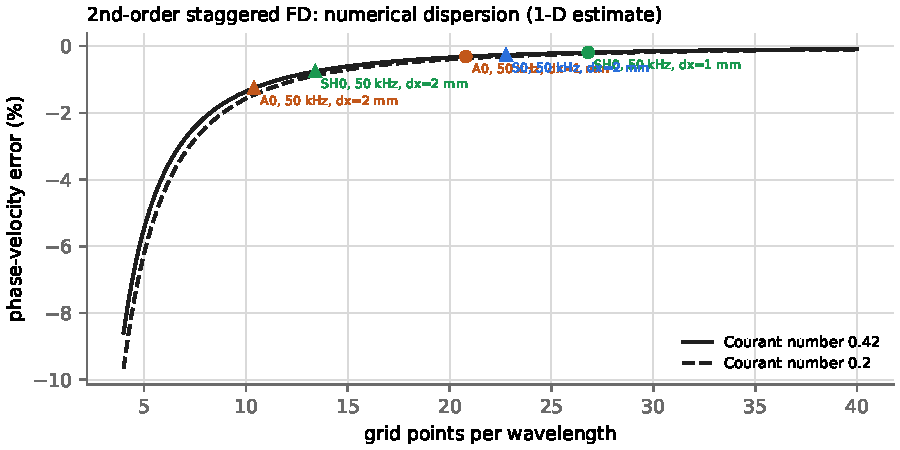
\includegraphics[width=0.72\textwidth]{grid_dispersion.pdf}
\caption{Phase-velocity error of the 2nd-order staggered scheme (1-D estimate) against points per wavelength, with
the shortest wavelengths of the three modes at 50~kHz for 0.5, 1 and 2~mm grids. In practice: plane stress converged
at 1~mm (1~mm vs 0.5~mm: 6\,\%), Mindlin needs 0.5~mm for 1~ms records (1~mm doubles the late-time error).}
\end{figure}

Time step: $\Delta t = 0.6\,\Delta x/(c_\text{max}\sqrt 2)$, with $c_\text{max}$ from the stiffest material (patch
stiffness or a stiff inclusion raise it). Remat stores the state only every 64 steps, which makes FWI gradients fit on
the GPU.

%======================================================================
\section{Summary: corrections and their effect}
\begin{table}[h]
\centering\small
\begin{tabularx}{\textwidth}{@{}p{3.2cm}LLp{3.2cm}@{}}
\toprule
Correction & Failure it addresses & How it is computed & Effect (from the summary report) \\
\midrule
S0 dispersion correction & constant S0 speed, phase error grows with distance & $v_p$ such that $c_p$ = exact S0 at 25~kHz & 0.38 $\to$ 0.27 (1~ms) \\
A0-matched $\kappa$ & Mindlin A0 1--2\,\% slow & $\kappa$ such that Mindlin A0 = exact A0 at 25 (39)~kHz & 0.87--0.99 $\to$ 0.16--0.20 \\
Damping & elastic model over-predicts far amplitudes & $a = \omega/Q$, Q = 40 & amplitude ratio flat 5--25~cm \\
Rigid body (instead of patch) & patch resonance & impulse projection on 3 rigid modes, physical mass/inertia & removes ringing \\
Effective footprint & full-size rigid footprint over-scatters & 6~mm, calibrated on Salvus & 0.28/0.23 $\to$ 0.16/0.11 (Salvus); LDV 0.31/0.33 \\
Source filter & unknown wavelet, delay, 2-D/3-D amplitude & closed form in frequency domain & used in every comparison \\
Windows, TV & residual model error & 300--500~$\mu$s; TV on the inverted maps & FWI artefacts 20.5 $\to$ 6.8~m/s \\
\bottomrule
\end{tabularx}
\end{table}

%======================================================================
\section{Recognising each failure in a residual}
\begin{table}[h]
\centering\small
\begin{tabularx}{\textwidth}{@{}LL@{}}
\toprule
Symptom & Likely cause \\
\midrule
Arrivals right but misfit near 1; a time stretch of a few percent fixes it & wave-speed error (uncorrected S0 or $\kappa$) \\
Misfit grows with time and number of reflections & frequency-dependent dispersion error (only partly corrected) \\
Shape difference constant with distance & source representation, not propagation \\
Rings radiating from an attached object at late times & patch resonance (use a rigid body) \\
Shadow behind an object too deep, strong front reflection & over-rigid / oversized footprint \\
Observed amplitude decays faster with distance than the model & attenuation missing \\
Same wave pattern and sign in in-plane and out-of-plane channels & LDV cross-talk, not in-plane motion \\
Residual concentrated within a few cm of the source & transducer near field / finite size \\
\bottomrule
\end{tabularx}
\end{table}

\end{document}
